\begin{figure}[h] %% zum drucken pdf verwenden
	\centering
  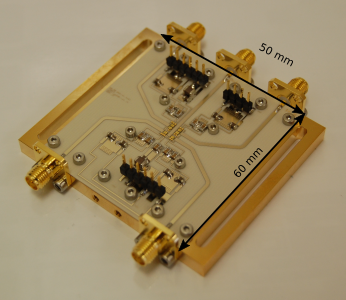
\includegraphics{Demonstrator_publish.png}
	\caption{Built demonstrator}
	\label{fig:Demonstrator}
\end{figure}
To the best of the author's knowledge, the worldwide first realised Riemann Pump in GaN technology is presented in Figure \ref{fig:Demonstrator}.\\

In this work a new concept of digital to analog conversion is investigated yielding an arbitrary waveform generator which can be used in the next generation of mobile communication.
For the development of this waveform generator, a proper concept is researched and simulated, a layout of the test circuit is developed and a first prototype is successfully built and measured.
The presented concept yields a waveform generator which is able to cover the frequency range from DC to \SI{6}{\giga \hertz}, which simulations confirmed.
With the help of this custom digital-to-analog converter, the actual conversion methods of digital to analog conversion are enhanced impressively.
The realised hybrid test circuit was built to prove the concept of a push-pull stage, functioning as a differential switch, providing a multi bit charge pump.
The multi chip solution is chosen to show the feasibility of generating different signals.
Simulations already demonstrates some draw backs and trade offs regarding the power consumption and the bandwidth limitation.
In addition to this some aspects are mentioned which influenced the signal quality.
In the design and realisation process custom drafts are developed to improve the heat transfer, while guarantee the proper functioning of the test circuit.
Furthermore some aspects are considered to reduce parasitic effects and undesired behaviour of the circuit.
After the assembly of the test circuit, different measurement concepts are prepared.
The digital input signal at four input ports required a special control strategy.
In addition, a proper output measurement strategy is described to illustrate the results.
The successful measurement of the built demonstrator finishes the proof of the demonstrated concept.
At last a conclusion sums up the results of the presented work and give an outlook for further improvements and investigations.





%\textbf{Agenda}
%\begin{enumerate}
%	\item literature survey
%	\item adaption of push-pull concept from Maksimovic (Talk at Fraunhofer IAF 06/2015)
%	\item GaN25 \gls{ab:gan} parameter simulation [S-parameter,ON/OFF switching voltage]
%	\item determine load impedance [input of PPA - GaN25 \gls{ab:hemt}
%	\item determine dimension of transistors
%	\item tuning schematic parameter for optimal simulation (special freq?)
%	\item enhancement/extension of 1-bit push-pull to 3-bit push-pull stage
%	\item digital input control voltage
%	\item determine eight slopes of the current sources in schematic 3-bit resolution
%	\item Riemanncode generation with MatLab; minimizing error
%	\item control schematic with theoretical input [Riemanncode]
%\end{enumerate}
%\vspace{1cm}
%\textbf{Problems}
%\begin{enumerate}
%	\item frequency dependent load impedance
%	\item absence of p-type transistor makes it hard to efficiently switch the high side transistor in the Gbps range
%	\item the heat spreading on the chip and substrate is critical
%	\item energy consumption may be very high (mainly switching losses)
%	\item the absence of accurate current sources makes it very hard to get a defined slope for the switching transistors.
%	\item theoretical slope generation very inaccurate
%	\item theoretical slope generation via shorted load  (R = \SI{1}{\ohm})
%	\item \textit {$\rightarrow$ slopes ambiguous}?	
%	\item \textit{$\rightarrow$ riemanncode generation not possible}?                                                                                                                                                                                                                                                                                                                                                                                                                                                                                                                                                                                                                                                                                                                                                                                                                                                                                                                                                                                                                                                                                                                                                                                                                                                                                                                                                                                                                                             
%\end{enumerate}
%\vspace{1cm}
%\textbf{Question}
%\begin{enumerate}
%%	\item mmW band much higher BW,Datarate,Spectrum - why use the old fashioned frequency bands from DC to 6GHz instead of using a couple of GHz?
%%	\begin{itemize}
%%		\item carrier frequencies of modern telecommunication standards are in the range of DC to 6 GHz
%%		\item Signal generation is done for the bandwidth of 0..\SI{6}{\GHz}, after that it could be mixed up to higher frequency bands like \SI{47}{\GHz} to \SI{53}{\GHz}
%%	\end{itemize}
%	\item trade off between BW and losses
%	\begin{itemize}
%		\item higher bandwidth means higher switching speed means higher losses due to the fact that the losses increase linear with the switching speed
%	\item higher frequencies means higher attenuation (e.g. weather condition, like rain)
%	\end{itemize}
%\end{enumerate}

\newpage
\chapter*{Zusammenfassung}

In dieser Arbeit wird ein neues Konzept der Digital-Analog-Umwandlung untersucht, ein Arbitrary Waveform Generator ergibt, die in der n\"achsten Generation der Mobilkommunikation verwendet werden k\"onnten.
auf \ SI {6} {\ giga \ Hertz}, die best\"atigt Simulationen: Diese Wellenform-Generator sollte den Frequenzbereich von \ gls {dc ab} abdecken k\"onnen.
Mit Hilfe dieser Multi-Bit-Aufl\"osung einer Ladungspumpe, die tats\"achlichen Umrechnungsmethoden Digital-Analog-Umwandlung kann verbessert werden. \\
Der realisierte Hybrid-Testschaltung wurde entwickelt, umgesetzt und bis zum Beweis das Konzept einer Push-Pull-Stufe gemessen, als Differenzschalter funktioniert, ein Multi-Bit-Ladungspumpe bereitstellt.
Die Multi-Chip-L\"osung wird die Machbarkeit des Ansatzes zu Beweis gew\"ahlt und bereits Kompromisse darstellen, die w\"ahrend der Arbeit auftreten. \\
Obwohl die Simulationen best\"atigt die Machbarkeit der Breitband-Frequenzbereich einige praktische Nachteile zu decken erw\"ahnt wurden, die den Frequenzbereich zu begrenzen.
Da die Erzeugung des Formsignals Welle am Ausgang der Schaltung, viel W\"arme erzeugt, zwei unterschiedliche Konzepte wurden nachgewiesen mit der W\"armeverteilung zu behandeln.
Da der Energieverbrauch der modernen Digital-Analog-Umwandlungen mit einer Aufl\"osung Mehrbit ist entscheidend ein Ansatz gew\"ahlt, der einen guten Wirkungsgrad liefert.